\section{Analysis: What Constitutes Improvement?}\label{sec:analysis}
\begin{figure}[!t]
\centering
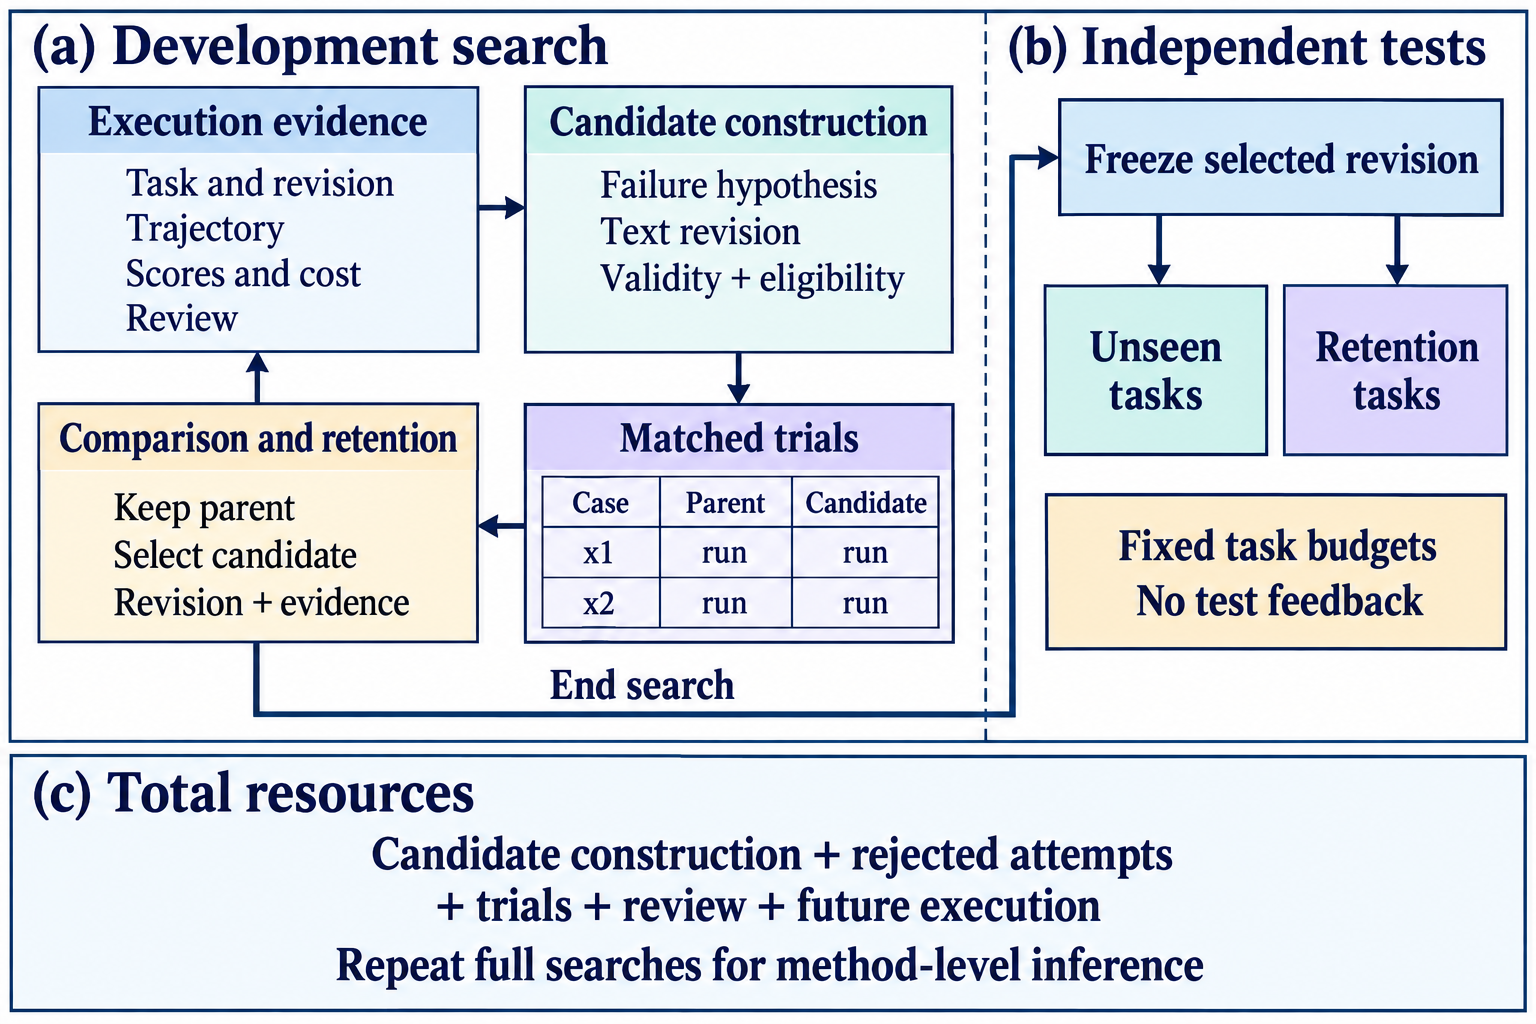
\includegraphics[width=\linewidth]{figures/evolution.png}
\caption{Evaluation design for retained organization revisions. Development trials support candidate construction and selection; frozen revisions are subsequently evaluated on separate future-task and retention sets. Trial cells depict comparisons, not measured results. All search and execution costs enter the accounting. Generalization over a search method requires independent search episodes and appropriate fresh partitions. This method diagram does not represent the protocol or outcomes of the preliminary Mission Base run in Section~\ref{sec:evaluation}.}
\label{fig:evolution}
\end{figure}

\subsection{Resource closure and revision isolation}
The inherited-reference constraint composes across retained revisions. If every transition satisfies Equation~\ref{eq:capability}, then, by transitivity of set inclusion, $\operatorname{Cap}(\mathcal O_v)\subseteq\operatorname{Cap}(\mathcal O_0)$ and likewise for base roles. Together with the frozen-file comparison, this bounds the resources an accepted candidate can introduce through this update path. It does not imply semantic safety: a changed instruction can misuse an existing tool, and a remote tool or externally resolved capability set can change without changing its reference.

Exact task binding also separates an update's intended unit of effect. Executions already bound to $h_v$ continue to identify $\mathcal O_v$; future tasks bound to $h_{v+1}$ identify the successor. This removes one source of attribution ambiguity, but it does not make the external environment stationary. Comparison contexts must still account for tool versions, model configuration, workspace state, and nondeterminism.

\subsection{Total value and amortization}
Let $q(\mathcal O,x)\in[0,1]$ measure task quality and let $c(\mathcal O,x)$ and $u(\mathcal O,x)$ measure execution cost and intervention time. For fixed nonnegative conversion weights $\lambda,\rho$, define per-task utility
\begin{equation}
U(\mathcal O,x)=q(\mathcal O,x)-\lambda c(\mathcal O,x)-\rho u(\mathcal O,x).
\label{eq:utility}
\end{equation}
Quality, cost, and time are also reported separately; the weights express an application-specific tradeoff rather than an intrinsic quality measure.

Suppose a revision has expected utility gain $g$ over its parent on the future task distribution, and the entire search and validation process costs $C_{\mathrm{search}}$ in the same utility units. Over $T$ tasks, its expected net advantage is
\begin{equation}
V_T=Tg-C_{\mathrm{search}},\qquad
V_T>0\ \Longleftrightarrow\ T>C_{\mathrm{search}}/g\quad(g>0).
\label{eq:amortization}
\end{equation}
This accounting identity explains why an improved task score is insufficient evidence of useful evolution. Search includes unsuccessful candidates, experiment planning, both trial arms, evaluator calls, and integrity review. When $g\leq0$, additional reuse cannot repay a nonnegative search cost under this stationary model. When tasks change over time, the relevant expression is $\sum_{t=1}^{T}g_t-C_{\mathrm{search}}$.

\subsection{Selection and unseen-task evidence}
A development winner is selected partly because of favorable observations. We therefore evaluate the frozen winner and parent on tasks withheld from candidate construction and selection. Let $d_i=q(\mathcal O',x_i)-q(\mathcal O_v,x_i)\in[-1,1]$ be the paired quality difference on independent held-out task units. Each $d_i$ can average multiple repeated executions within the task; those repeats do not increase the number of independent tasks.

Conditional on the fixed organizations, Hoeffding's inequality gives \citep{hoeffding}
\begin{equation}
\Pr\!\left(\left|\bar d-\mathbb E\bar d\right|\geq\epsilon\right)
\leq 2\exp(-n\epsilon^2/2),\qquad
\epsilon(n,\alpha)=\sqrt{\frac{2\log(2/\alpha)}{n}}.
\label{eq:bound}
\end{equation}
This conservative bound remains valid for nonidentical independent task distributions, with $\mathbb E\bar d$ interpreted as their average effect. A claim about a target population additionally requires representative sampling. Repository or source-document dependence requires defining the independent unit at that cluster level.

If $K$ candidates are all fixed before inspecting the same held-out set, a union bound replaces $\log(2/\alpha)$ with $\log(2K/\alpha)$ for simultaneous intervals. This finite-family bound does not justify adaptively generating new candidates from held-out results. Such feedback converts the set into development data and requires a fresh test set. At $K=1$ and $\alpha=0.05$, a worst-case half-width of $0.10$ requires $n\geq738$ independent units; a small pilot cannot establish a precise population-level improvement. The inequality is a standard statistical tool, not a new learning guarantee. Its estimand is the effect of the frozen revision pair. It does not average over the random search process that produced the candidate.
